% !TEX root = ../document.tex

\chapter{现阶段发展及应用情况}

\section{“铱星二代”系统}

\begin{figure}[htbp]
\centering
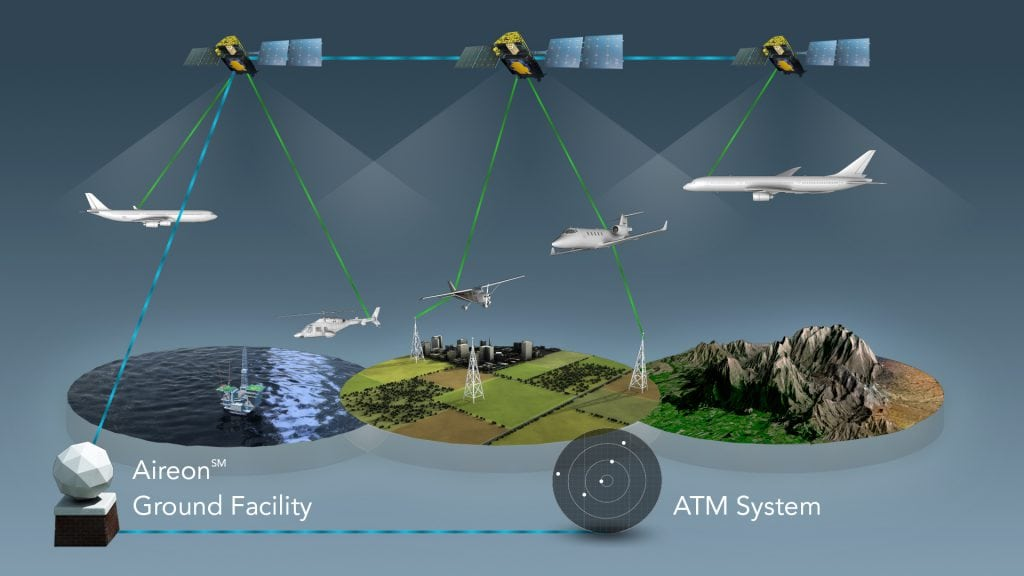
\includegraphics[width=15cm]{pic/Aireon_GlobalSpaceBasedADSB_Coverage_Diagram-1024x576.jpg}
\caption{Aireon 天基 ADS-B 系统布局原理}
\label{fig:Aireon_GlobalSpaceBasedADSB_Coverage_Diagram}
\end{figure}

\begin{figure}[htbp]
\centering
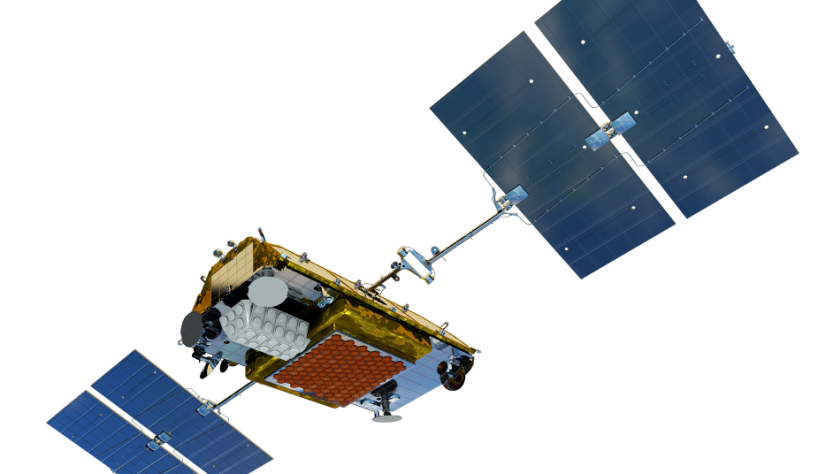
\includegraphics[width=13cm]{pic/IMG_Iridium-Satellite_NEXT-Satellite-Vehicle_HR_FEB16-clip-833x474.png}
\caption{第二代“铱星”卫星}
\label{fig:IMG_Iridium-Satellite_NEXT-Satellite-Vehicle}
\end{figure}

\begin{figure}[htbp]
\centering
\begin{minipage}[t]{0.48\textwidth}
\centering
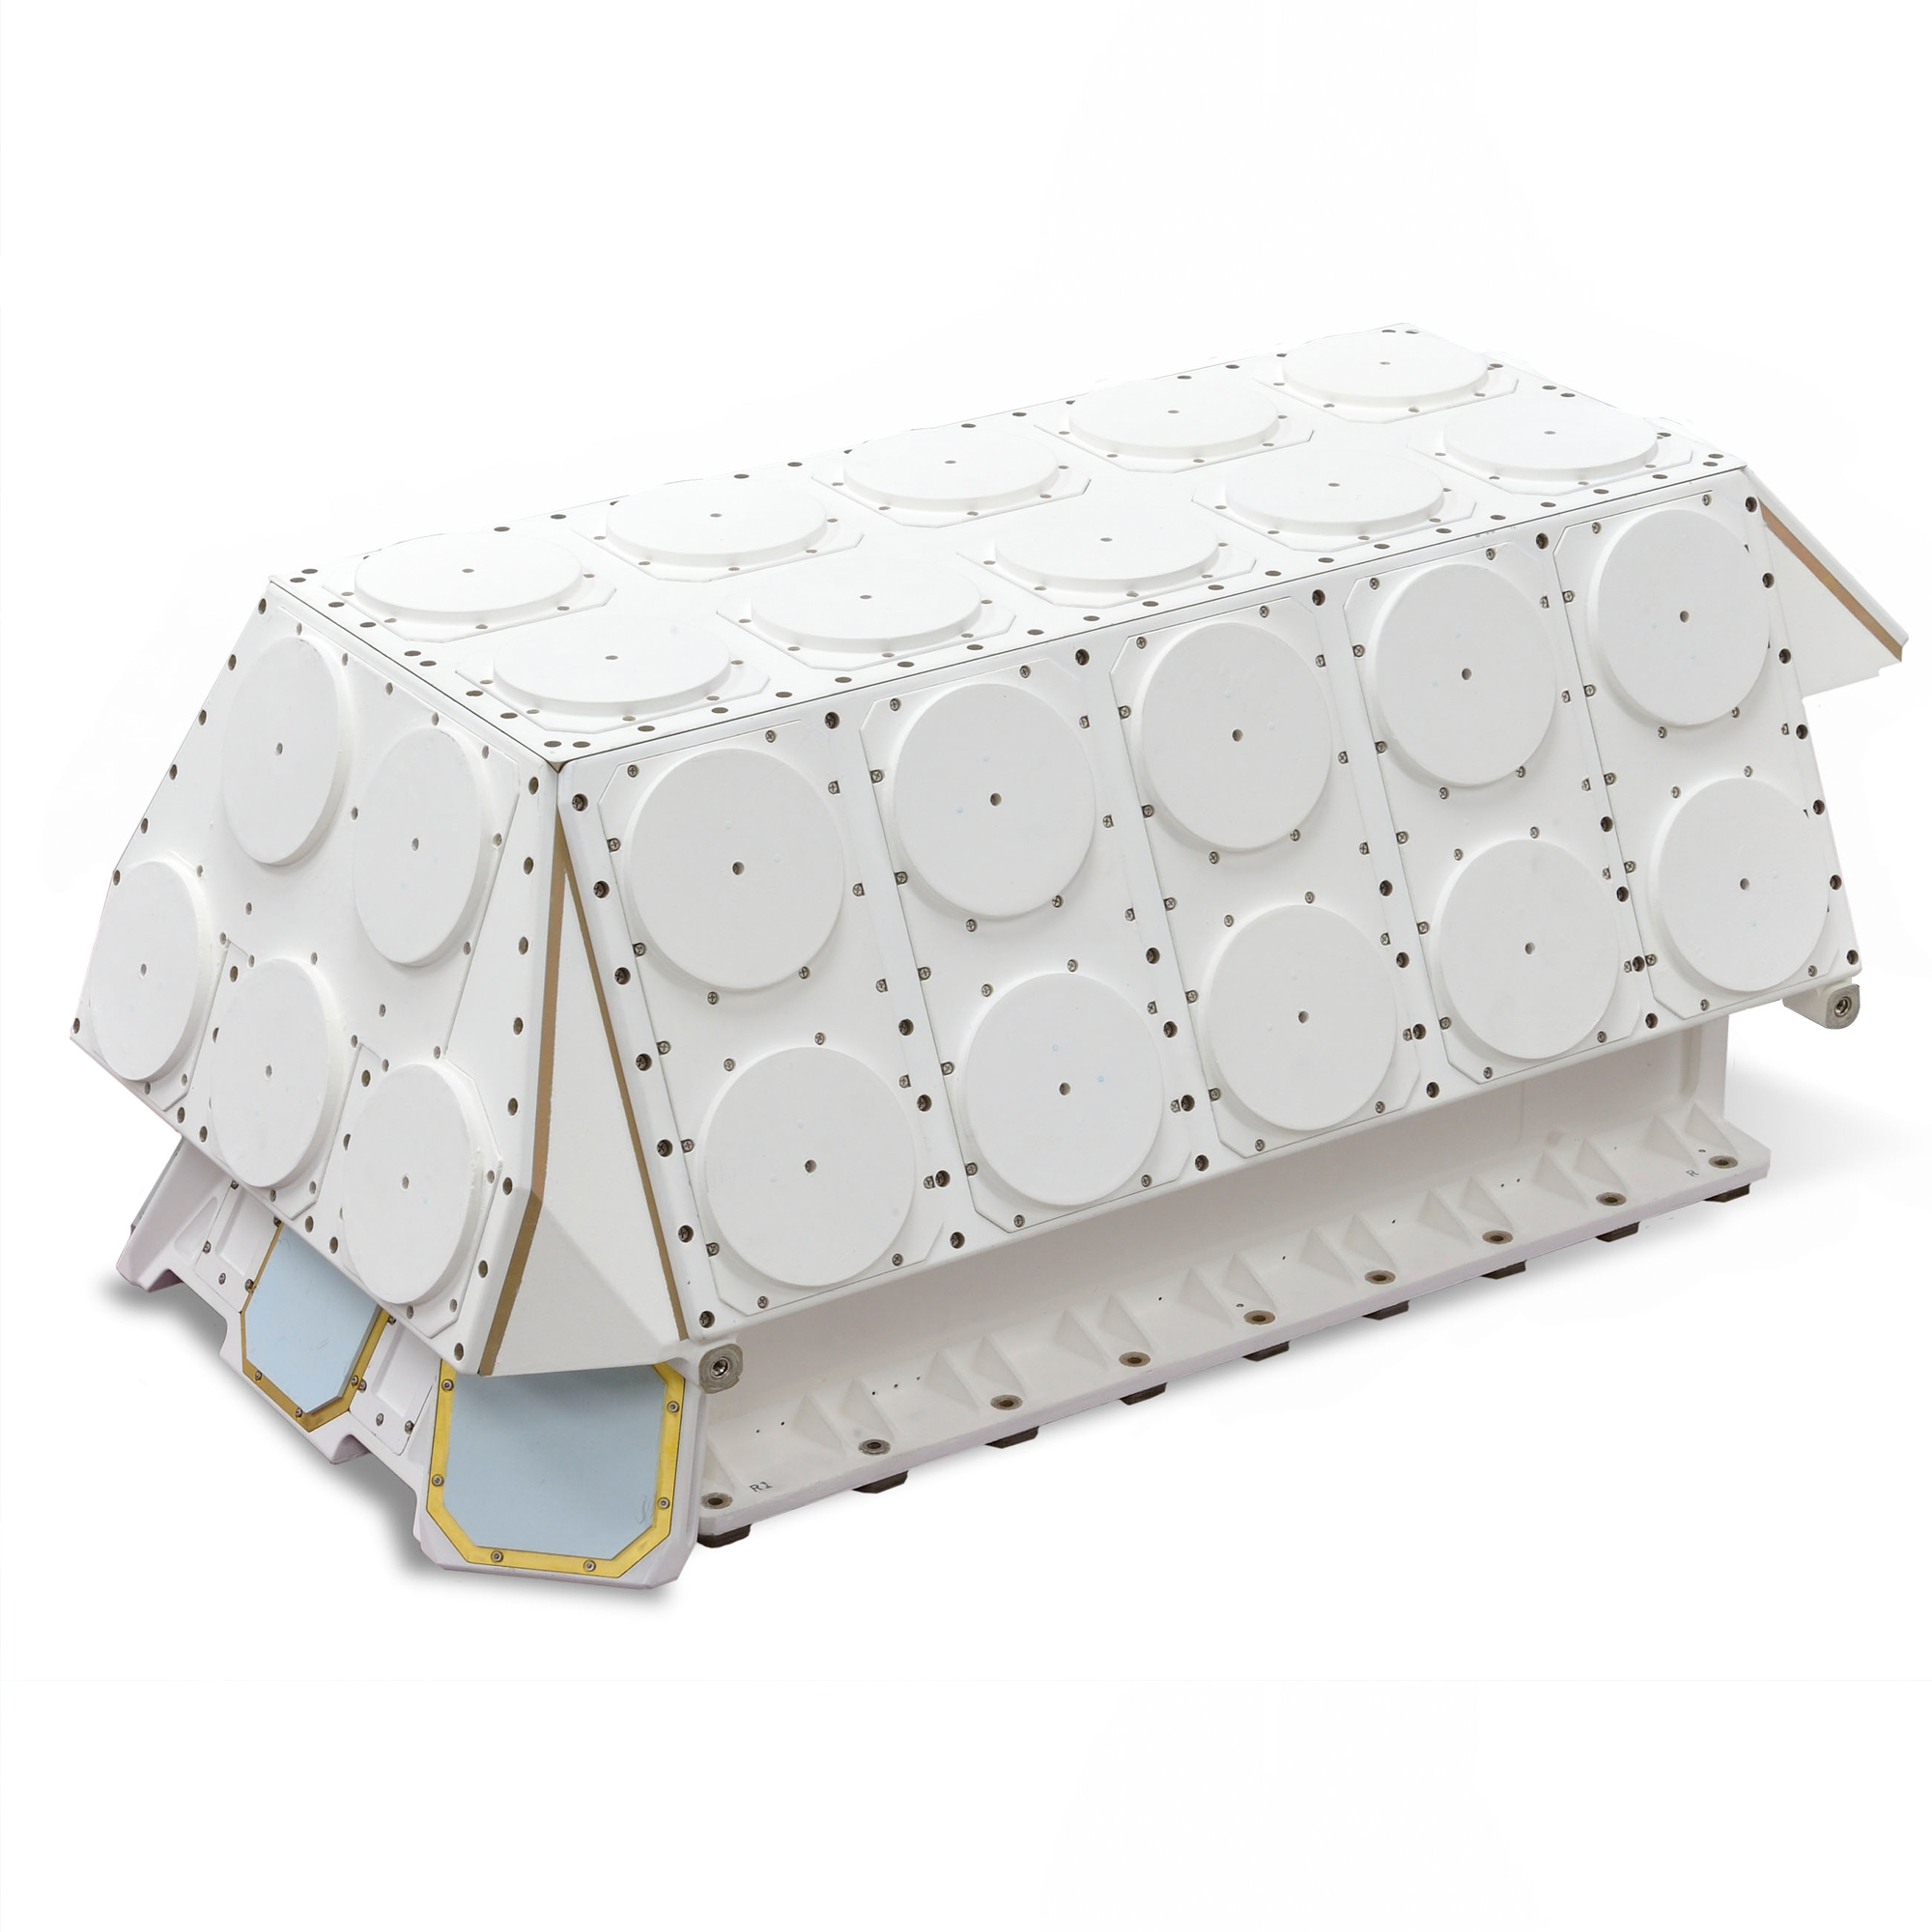
\includegraphics[width=6.5cm]{pic/Appstar_with_Base_2000x2000.jpg}
\caption{ADS-B 载荷}
\label{fig:Appstar_with_Base}
\end{minipage}
\begin{minipage}[t]{0.48\textwidth}
\centering
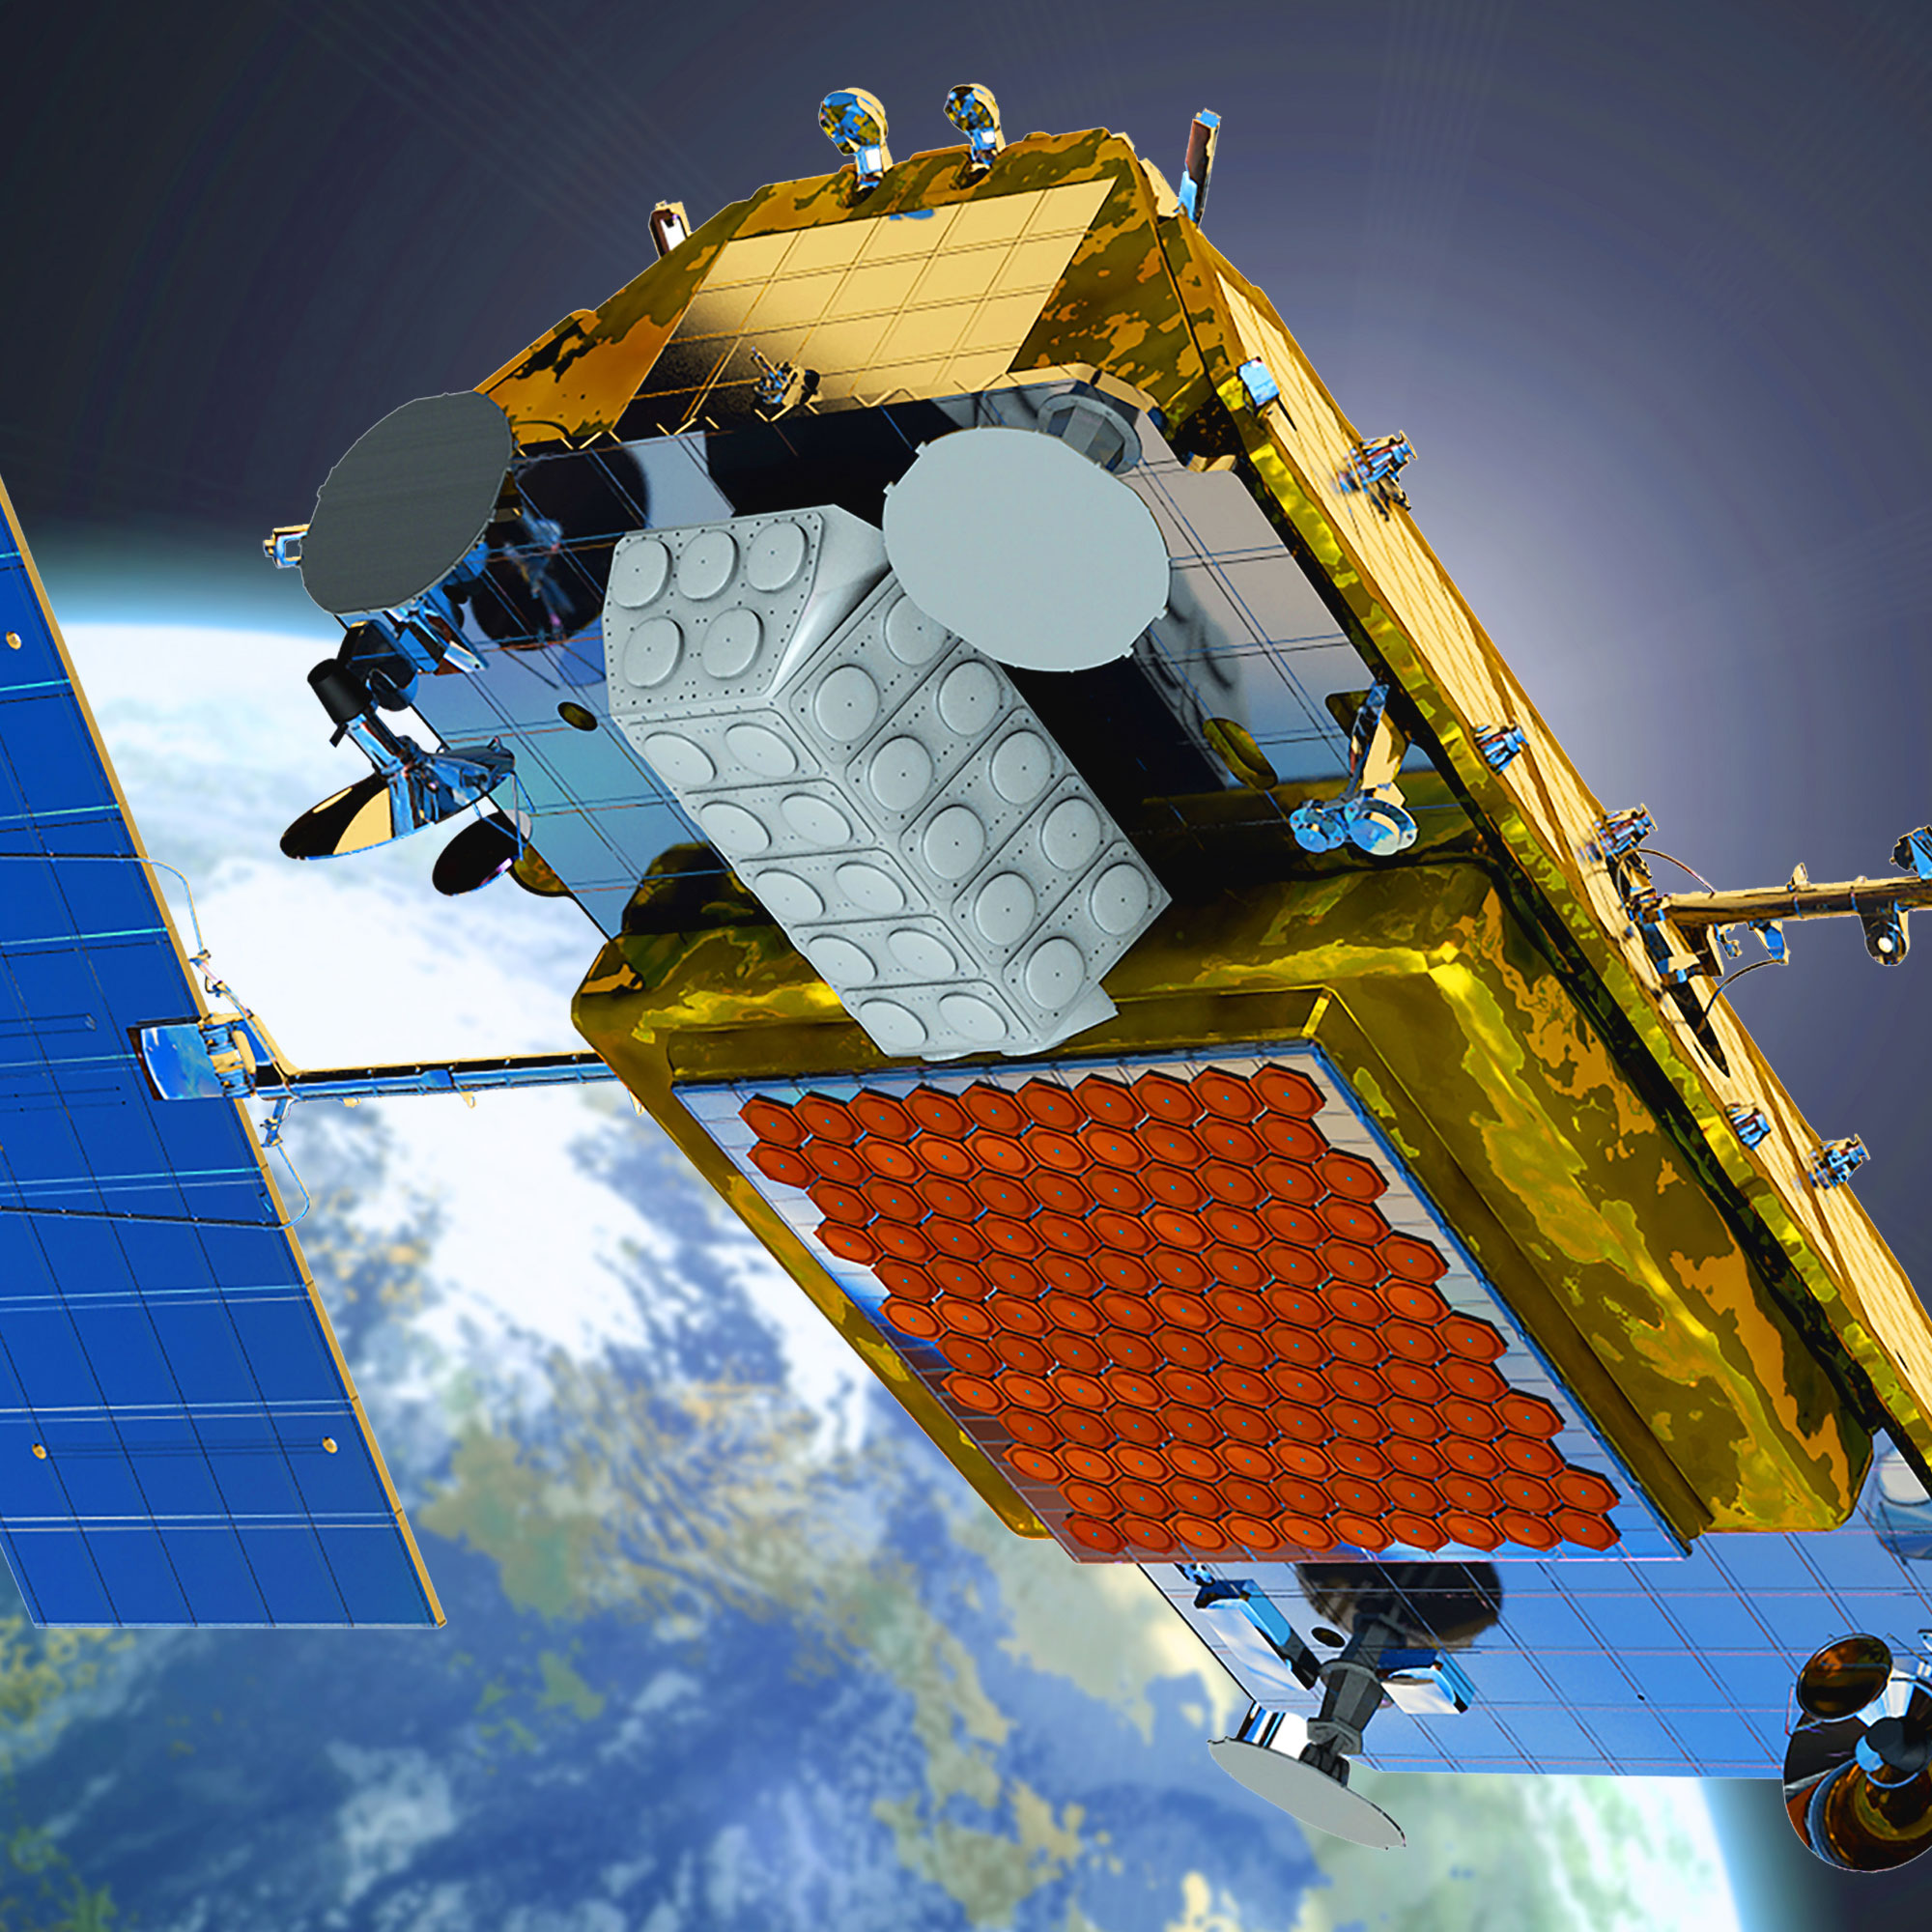
\includegraphics[width=6.5cm]{pic/reconfigurable_multimission_payloads_v2_web.jpg}
\caption{ADS-B 载荷搭载方式}
\label{fig:reconfigurable_multimission_payloads}
\end{minipage}
\end{figure}

\section{“全球星二代”系统}

根据\url{www.ads-b.com}网站给出的说法,他们将天基 ADS-B 系统称为 ADS-B 链路增强系统(ADS-B Link Augmentation System),简称为“ALAS”。通过该系统,地球上任何地方的任意一架飞机可以被实时地安全追踪。

\renewcommand\arraystretch{1.5}
\begin{table}[htbp]
\centering
\caption{使用全球星卫星的 ALAS 系统端到端测试性能}
\label{tab:alas-paras}
\begin{tabular}[b]{|p{4cm}<{\raggedleft}|p{11cm}<{\raggedright}|}
\hline
\textbf{适用性
(Applicability)} &
ALAS 是一种简单、质量轻、低成本的外围设备,可与现有的任何 1090ES 或 UAT 电子设备配合使用,保证正常的空-地和地-空 ADS-B 传输不会中断。ALAS 还旨在与任何国家现有的 ADS-B 地面基础设施兼容\\
\hline
\textbf{覆盖范围(
Coverage Area)} &
到 2016 年,100\% 覆盖美国本土(CONUS)、GOMEX、加勒比海(Caribbean)、北大西洋(NAT)和北太平洋(NOPAC);到 2019 年,100\% 覆盖剩余地区\\
\hline
\textbf{可用性(
Availability)} & 到 2016 年,可用性为 99.99\%;到 2019 年,可用性为 99.999\% \\
\hline
\textbf{容量(
Capacity) }& 每架卫星可容纳大于 3000 架飞机(approx 1,800sm diameter)\\
\hline
\textbf{时延(
Latency)} &  从飞机到地面小于 200 毫秒;从端到端小于 300 毫秒 \\
\hline
\textbf{更新率(
Update Rate)} & 1 秒 \\
\hline
\textbf{完整性(
Integrity)} & 10E-6 \\
\hline
\textbf{精度(
Accuracy)} &
UTC 时制下,在 98\% 的时间里,相同目标的 射频视距(RF line-of-sight)导出位置和天基 ALAS 导出位置之间的显示位置差异小于 50 英尺\\
\hline
\textbf{安全性(
Security)} & 独一无二的安全。ALAS 与每架飞机建立了独特的双向连接,可以抵抗入侵、干扰或欺骗,是唯一的可以轻松加密的 ADS-B 形式。简单的防篡改设计还可以包括一个自供电备用系统,该系统将在未经授权而关闭飞机的主 ADS-B 转发器的情况下继续广播飞机的位置 \\
\hline
\textbf{可扩展性(
Scalability)}  & 高。系统架构的成本相对较低且简单,通过增加更多卫星和/或地面站,可以提高覆盖范围,可用性和容量 \\
\hline
\textbf{部署(
Deployment)} & 马上准备好。该技术已经过超过 100 小时的飞行测试。Globalstar 在过去两年中发射了 24 颗新的第二代 ALAS 卫星。Essential Services could be deployed as early as 3Q2016 and Critical Services NLT 2019\\
\hline
\textbf{成本(
Cost)} & 低。由于 ALAS 不需要新的卫星或太空中的其他技术,因此 ANSP 的买入和重复成本很小。它还可以与现有的 ADS-B 地面基础设施轻松连接。The price point for Part 121 avionics is less than \$40k and installation should be in the 20-25 MH range for most commercial aircraft. \\
\hline
\end{tabular}

\end{table}